\subsection{High-Pass Filter}
\index{High-Pass Filter}
\index{Filters!High-Pass Filter}

$Revision: 1.7 $

As the low-pass filter, the high-pass filter (e.g. is in \xf{fig:high-pass})
has been realized on top of the FFT Filter,
in fact, it is the opposite to low-pass filter, and filters out
frequencies before 2853~Hz.
The implementation of the high-pass filter can be found in
\api{marf.Preprocessing.FFTFilter.HighPassFilter}.

\begin{figure}
	\centering
	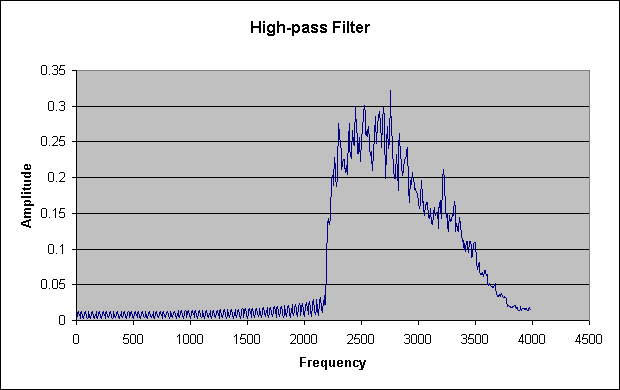
\includegraphics[width=400pt]{../graphics/graphs/high-pass-filter.png}
	\caption{High-pass filter applied to aihua5.wav.}
	\label{fig:high-pass}
\end{figure}

% EOF
